\chapter{Dataset and evaluation metrics}
\label{Dataset}

In the Section~\ref{dataset} we describe the dataset which is used for training and evaluation purpose for our task of the human pose estimation.
In Section~\ref{evaluation-metric} we define the evaluation metric for the aforementioned task.

\section{Dataset}
\label{dataset}

The most common datasets for the task of human pose estimation from point clouds are ITOP \parencite{haque_towards_2016} and EVAL \parencite{liu_point_2020}. In this work we concentrate on ITOP dataset since it's more widely used \parencite{shotton_real-time_2011,ho_yub_jung_random_2015,carreira_human_2016,chen_pose_2020,moon_v2v-posenet_2018} thus has more related works for results' comparison.

\subsection{ITOP}
ITOP dataset was first released in the work of \cite{haque_towards_2016}. The dataset comprises depth images of people in different poses. An example of the depth map from the dataset is shown in Figure~\ref{img:dataset-points-with-depth}. 

The snapshots of poses are taken from two different viewpoints: the side view, and the top view. In side view, the camera faces a person directly in front (the whole body is seen). In the top view, the camera is placed above the person's head and shots the view from the top (torso usually occluded by shoulders and arms).

The dataset is collected inside of the room thus some furniture items appear in the dataset. Due to excess obstacles in the field of view of the camera, we apply preprocessing pipelines to extract only human point clouds. The pipeline is described in Section~\ref{Data-preparation}. Figures \ref{img:dataset-human-examples-front-view} and \ref{img:dataset-human-examples-top-view} show examples of side and top views respectively.

The 3-dimensional $(x,y,z)$ coordinates are relative to sensor's position. The distance is measured in meters. Thus, if $x$ coordinate hasa  value of $2$, it means that the point is 2 meters right relatively to the sensor's $(0, 0, 0)$ reference point.

Ground truths consist of  15 joint key point coordinates - head, neck, shoulders, elbows, hands, torso, hips, knees, and feet. An example of named joints is shown in Figure~\ref{img:dataset-example-joints}. Table~\ref{tab:dataset-statistics} covers general statistics on dataset size.

\begin{table}
    \caption{General statistic for ITOP dataset}
    \label{tab:dataset-statistics}
    \centering
    \begin{tabular}{l l l l}
    \toprule
    \tabhead{View} & \tabhead{Split} & \tabhead{Frames} & \tabhead{People} \\
    \midrule
        side & train & 39,795 & 16 \\
        side & test  & 10,501 & 4  \\
        top  & train & 39,795 & 16 \\
        top  & test  & 10,501 & 4  \\
    \bottomrule\\
    \end{tabular}
\end{table}

\begin{figure}[htbp]
    \centerline{\includegraphics[scale=.17]{Figures/points-with-depth.png}}
    \caption{Four examples of depth images from ITOP dataset. The darker the color the closer it's located to the camera}
    \label{img:dataset-points-with-depth}
\end{figure}

\begin{figure}[htbp]
    \centerline{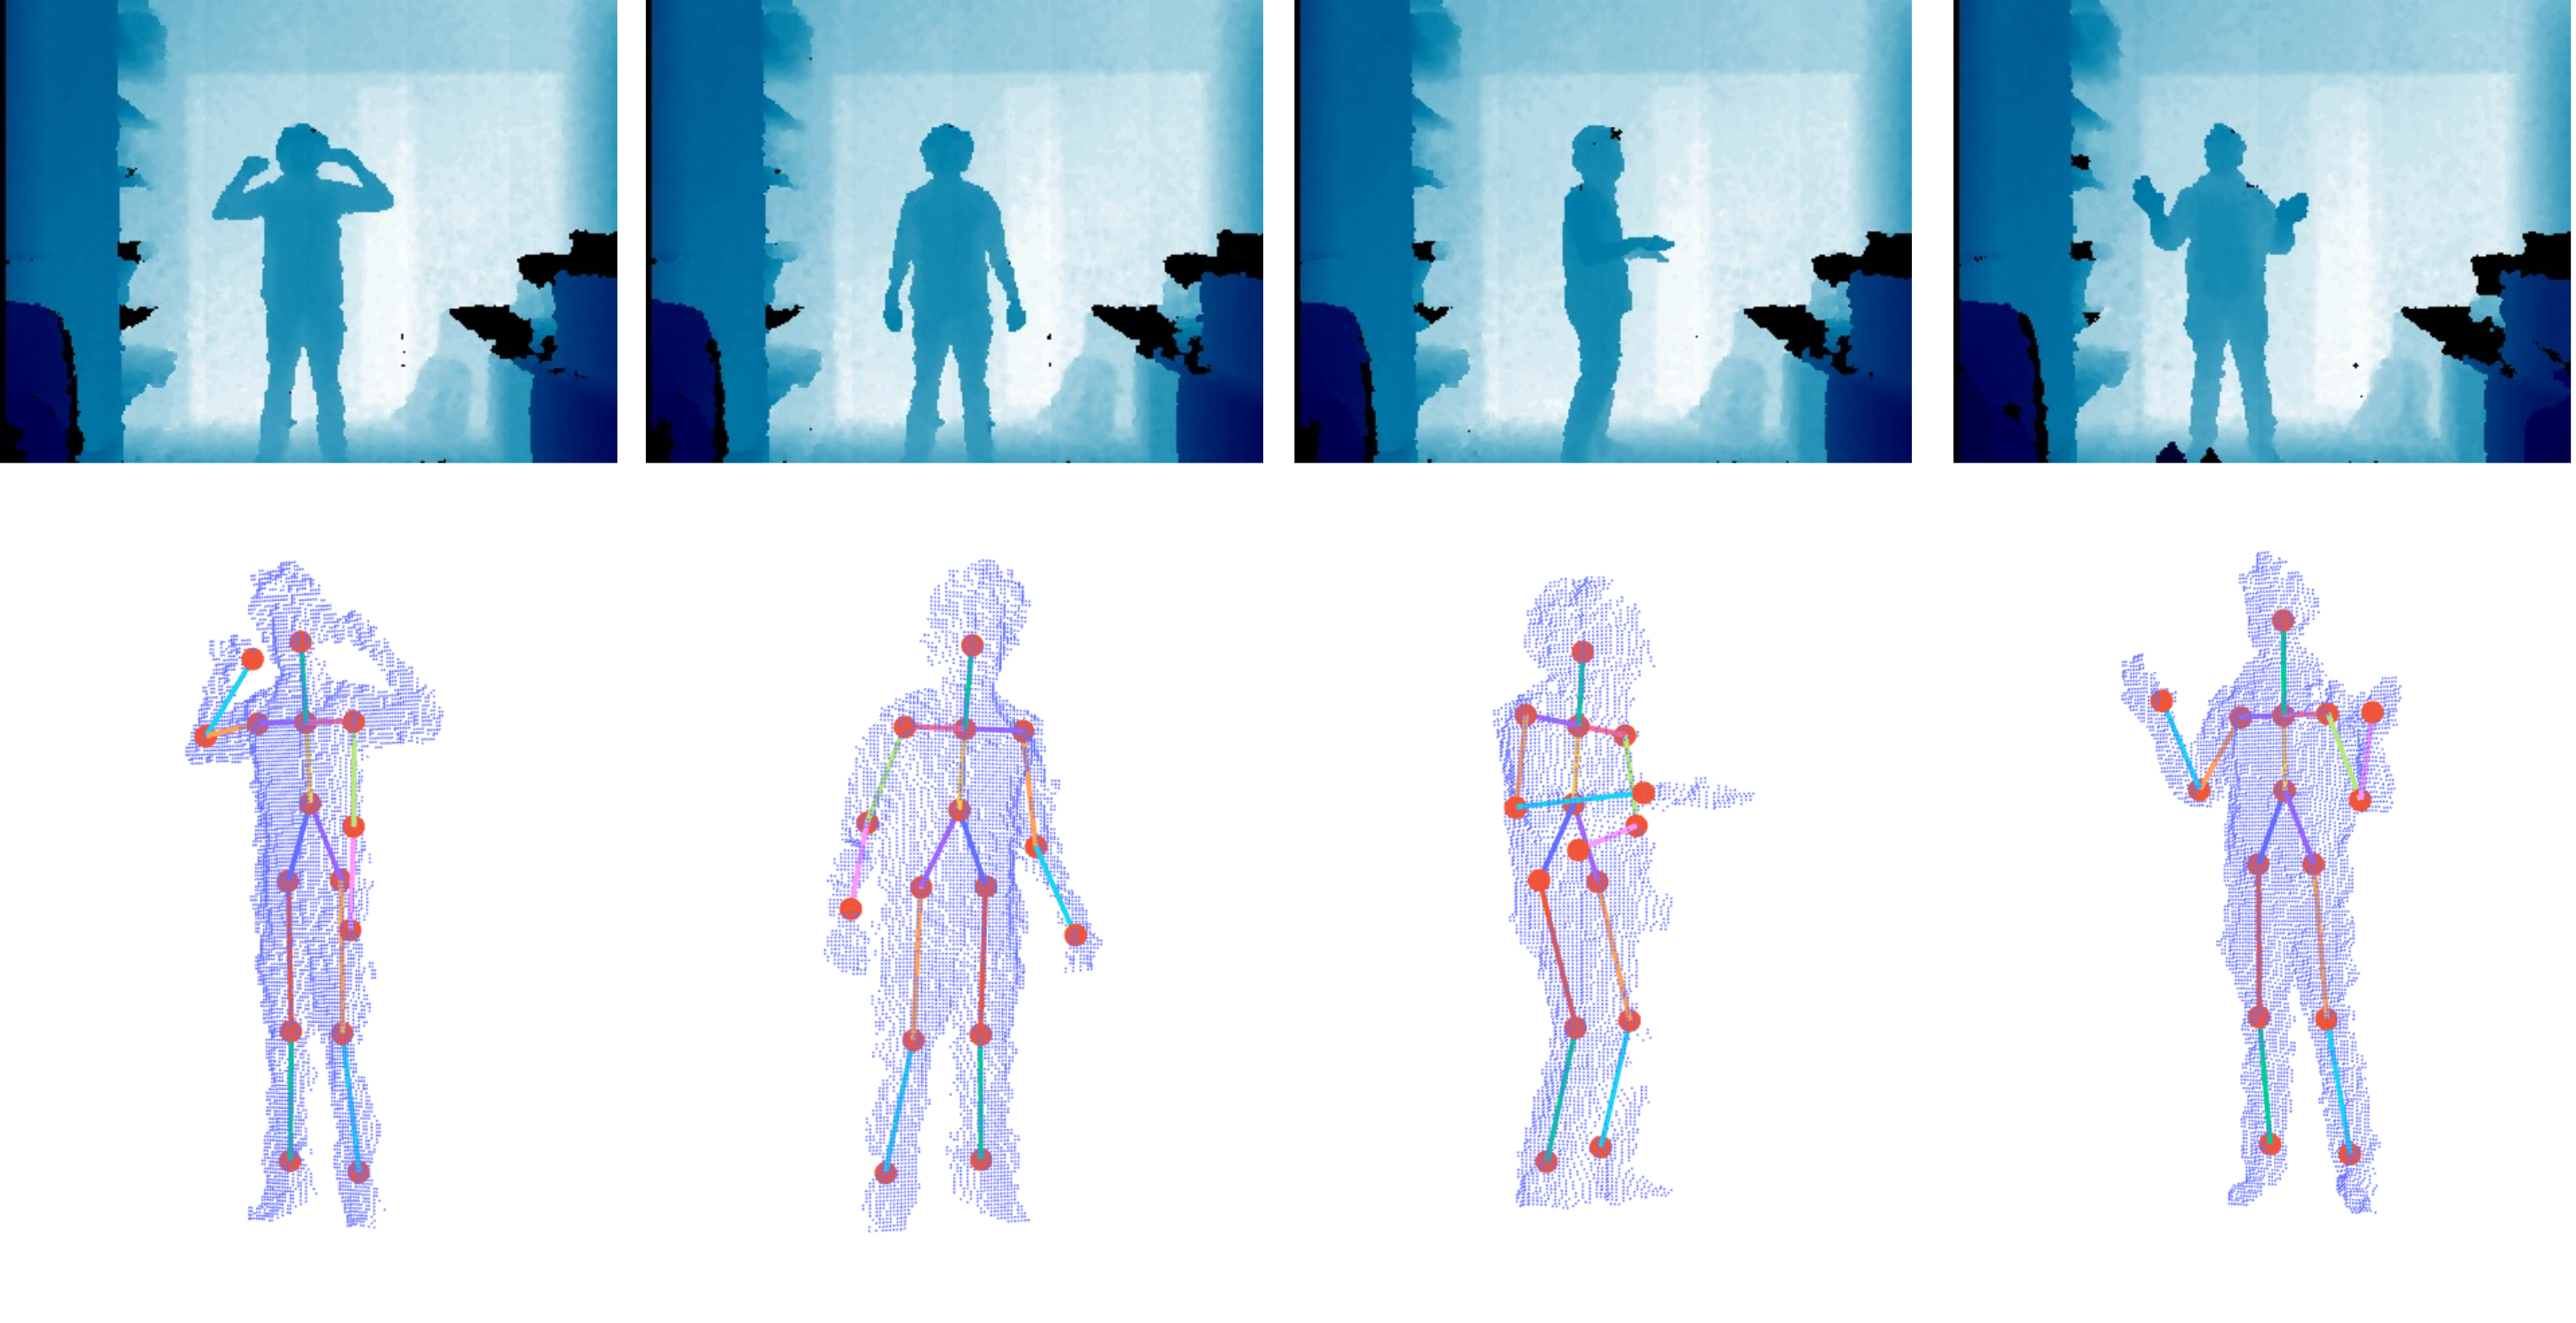
\includegraphics[scale=.15]{Figures/dataset examples - side view.png}}
    \caption{Four examples of front view subset of ITOP. Upper images are depth representation. Bottom images show human point clouds (blue) with key joints (red)}
    \label{img:dataset-human-examples-front-view}
\end{figure}

\begin{figure}[htbp]
    \centerline{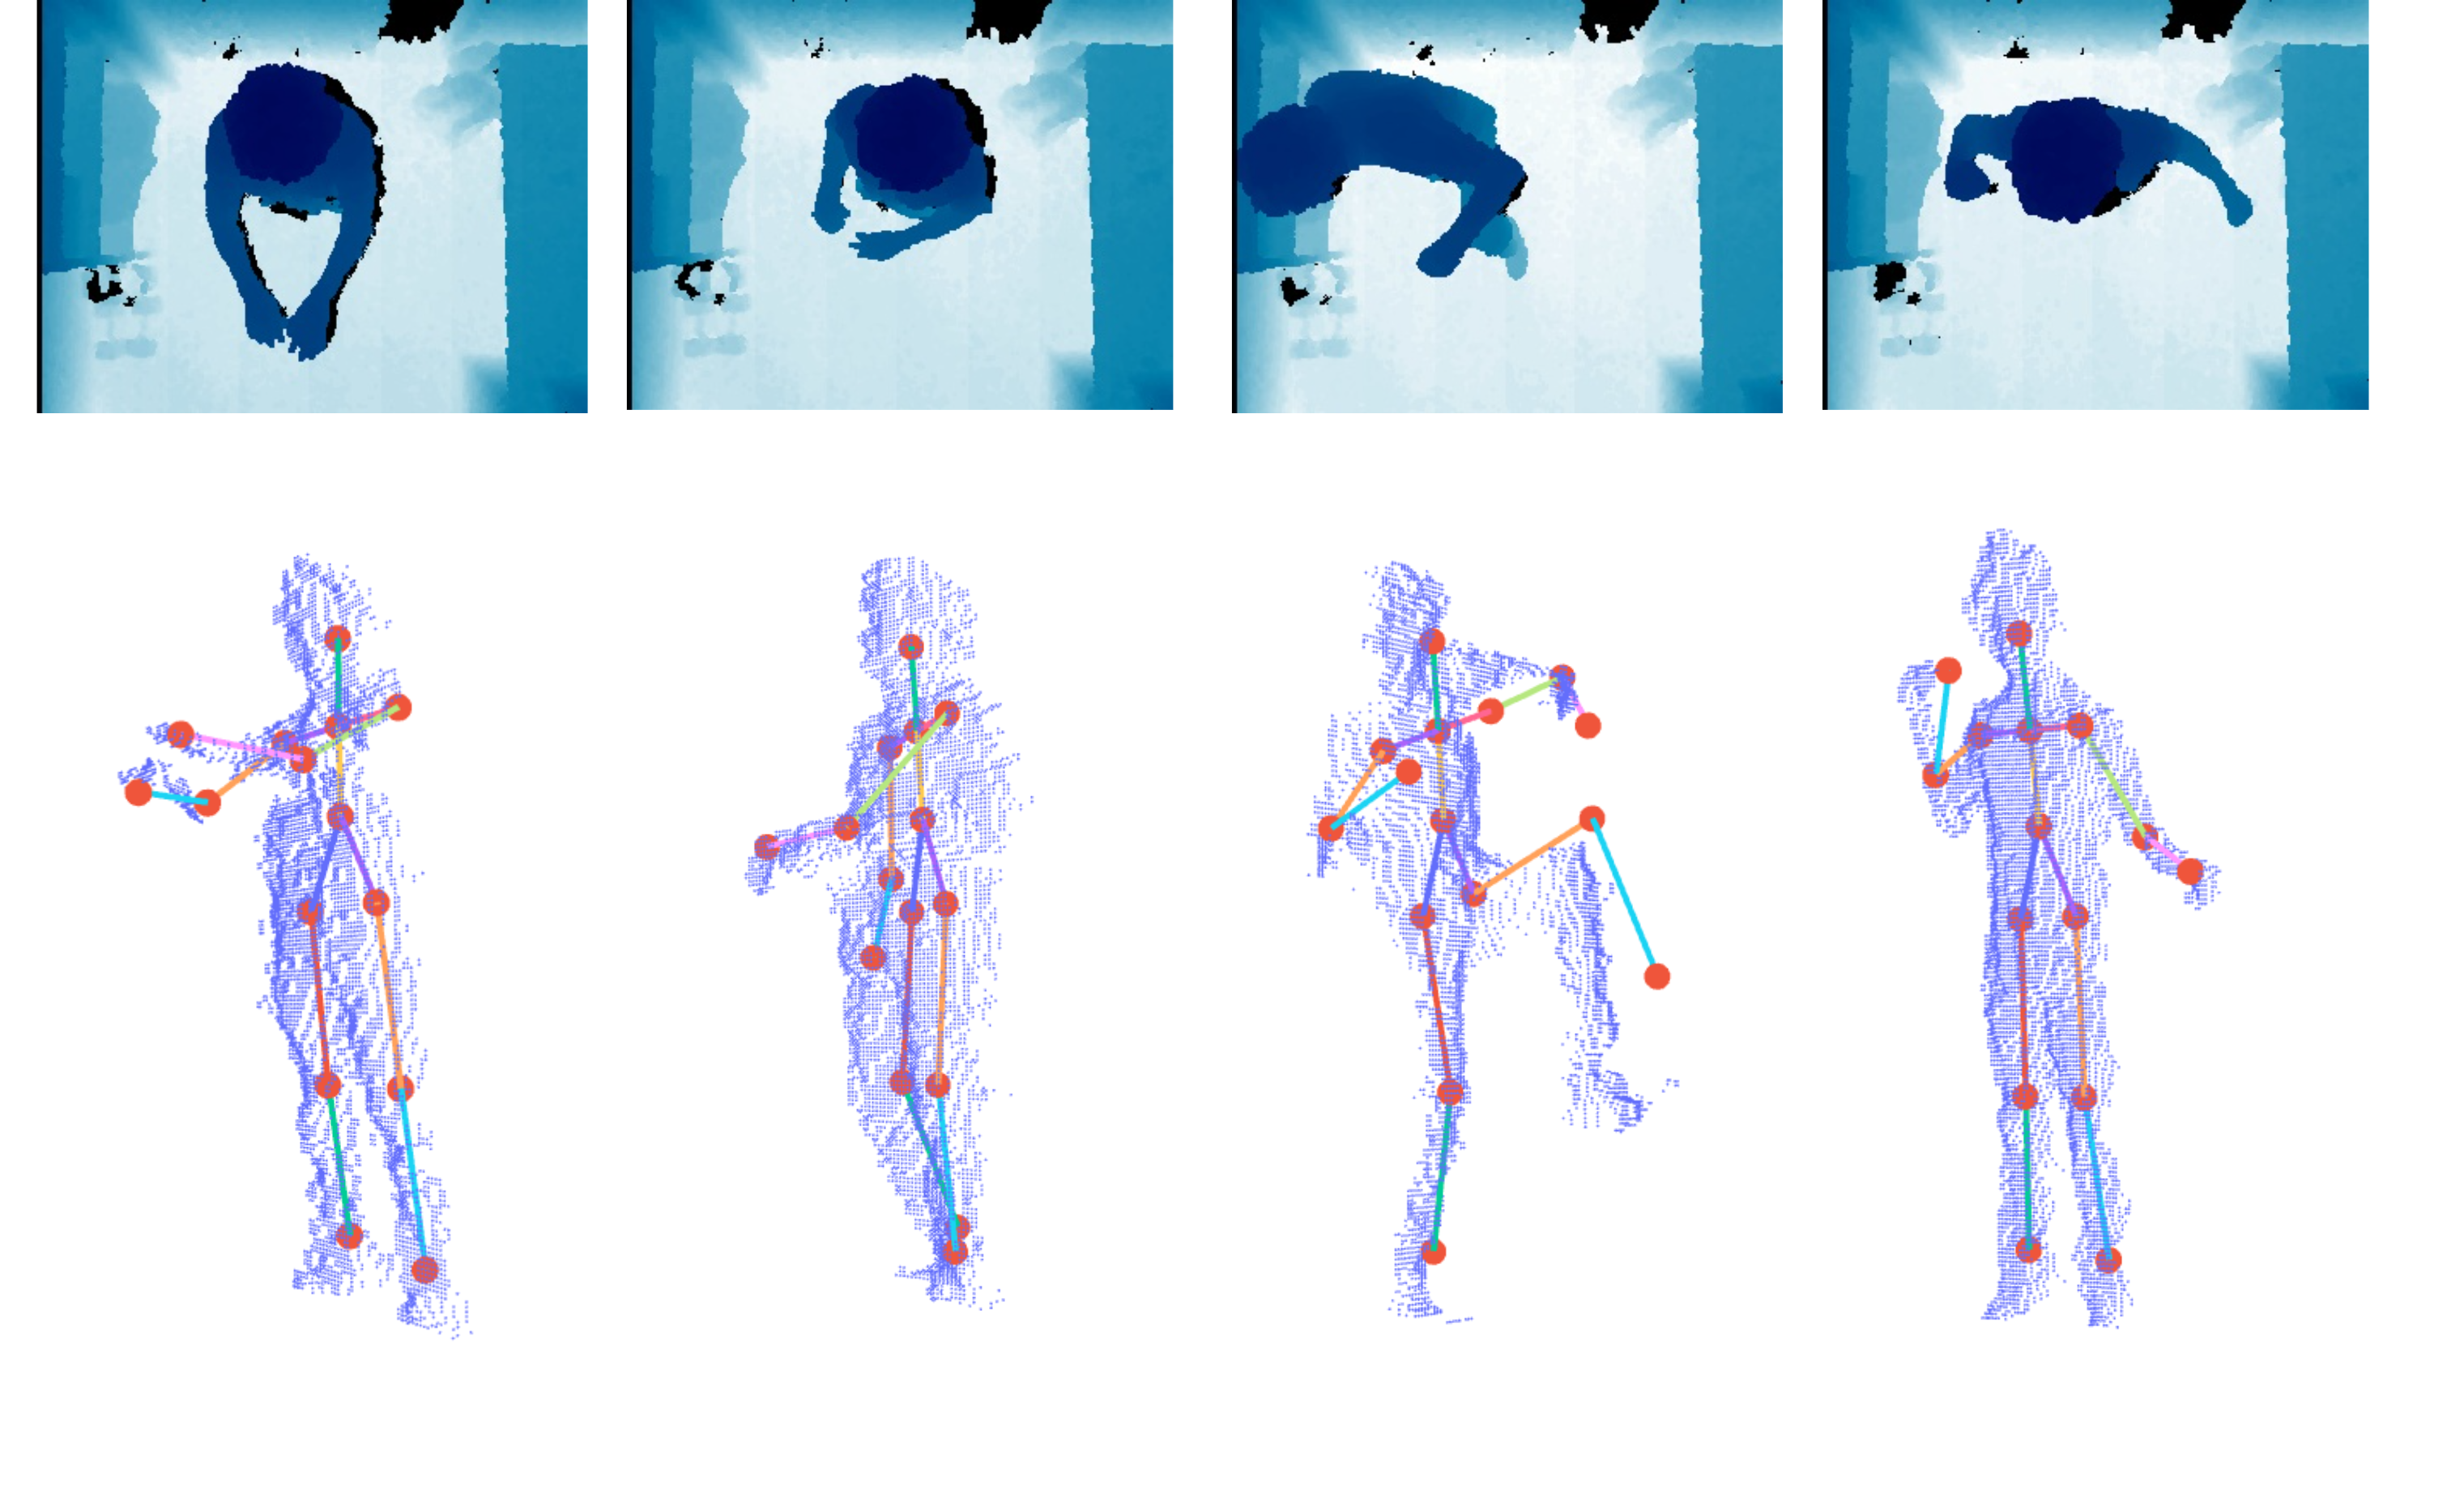
\includegraphics[scale=.15]{Figures/dataset examples - top view.png}}
    \caption{Four examples of top view subset of ITOP. Upper images are depth representation. Bottom images show human point clouds (blue) with key joints (red)}
    \label{img:dataset-human-examples-top-view}
\end{figure}

\begin{figure}[htbp]
    \centerline{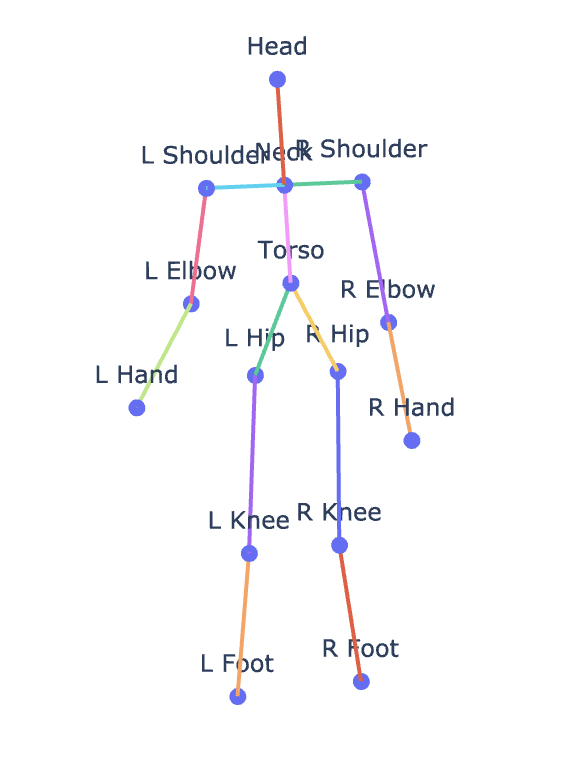
\includegraphics[scale=0.8]{Figures/dataset-example-joints.png}}
    \caption{Example of key joints with names from ITOP dataset}
    \label{img:dataset-example-joints}
\end{figure}

\section{Evaluation metric}
\label{evaluation-metric}
Since we are working on the regression task, we use mean Average Precision (mAP) as our main metric of the model's performance. The ground truths are coordinates of key human joints (denoted as $J$). The output of the regression model is also joints' coordinates of the same size as $J$ (denoted as $\hat{J}$).

To be able to compare our results with the work of others \parencite{haque_towards_2016,moon_v2v-posenet_2018,guo_towards_2017} we use the same approach of calculation of $AP$ using $10 \ cm$ distance threshold. By this rule (Formula~\ref{eqn:dataset-metric-ap}) the predicted joint is considered correctly detected if the $L_2$ distance to ground truth is equal or less that $10 \ cm$. The resulting $mAP$ is calculated by averaging $AP$ by the number of samples (Formula~\ref{eqn:dataset-metric-map}).

For further convenience, we will also apply the plot with $mAP$ values for distances from $0 \ cm$ to $100 \ cm$ (Example in Figure~\ref{img:example-map}).

\begin{equation}
\label{eqn:dataset-metric-ap}
AP(J, \hat{J})=\left\{\begin{array}{ll}
    1, & \lVert J - \hat{J} \rVert <10 \mathrm{~cm} \\
    0, & \text { otherwise }
\end{array}\right.
\end{equation}

\begin{equation}
\label{eqn:dataset-metric-map}
    mAP=\frac{\sum_{i=0}^{M} A P\left(J_{i}, \hat{J_{i}}\right)}{M}
\end{equation}

\begin{figure}[htbp]
    \centerline{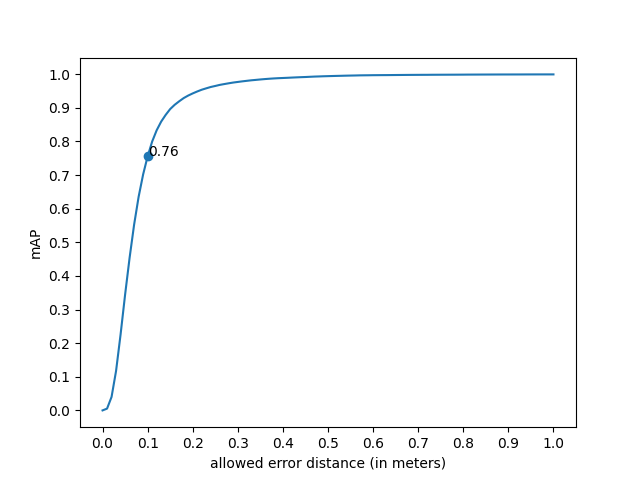
\includegraphics[scale=.6]{Figures/example-map.png}}
    \caption{Example of the mAP plot. On the X axis - allowed distance between predicted and ground truth coordinates to be considered as a right detection. On the Y axis - mean Average Precision for given distance. The values for $\textbf{distance} = 10 \ cm$ is highlighted on the plot.}
    \label{img:example-map}
\end{figure}